\chapter{Methods}

\section{Registration}
``Image registration is the process of overlaying two or more images
of the same scene taken at different times, from different viewpoints,
and/or by different sensors. It geometrically align two images --the
reference and sensed images.''\cite{zitova}

``Image registration is a crucial step in all image analysis tasks in
which the final information is gained from the combination of various
data sources like in image fusion, change detection, and multichannel
image restoration.''\cite{zitova}\\


The following images show a comparison of two volumes taken of the
same patient at different times. Figure \ref{before_reg} shows the
image comparison before performing affine registration. Figure
\ref{after_reg} shows the comparison of images after the registration
has been done.

\begin{figure}[htb]
  \centering
  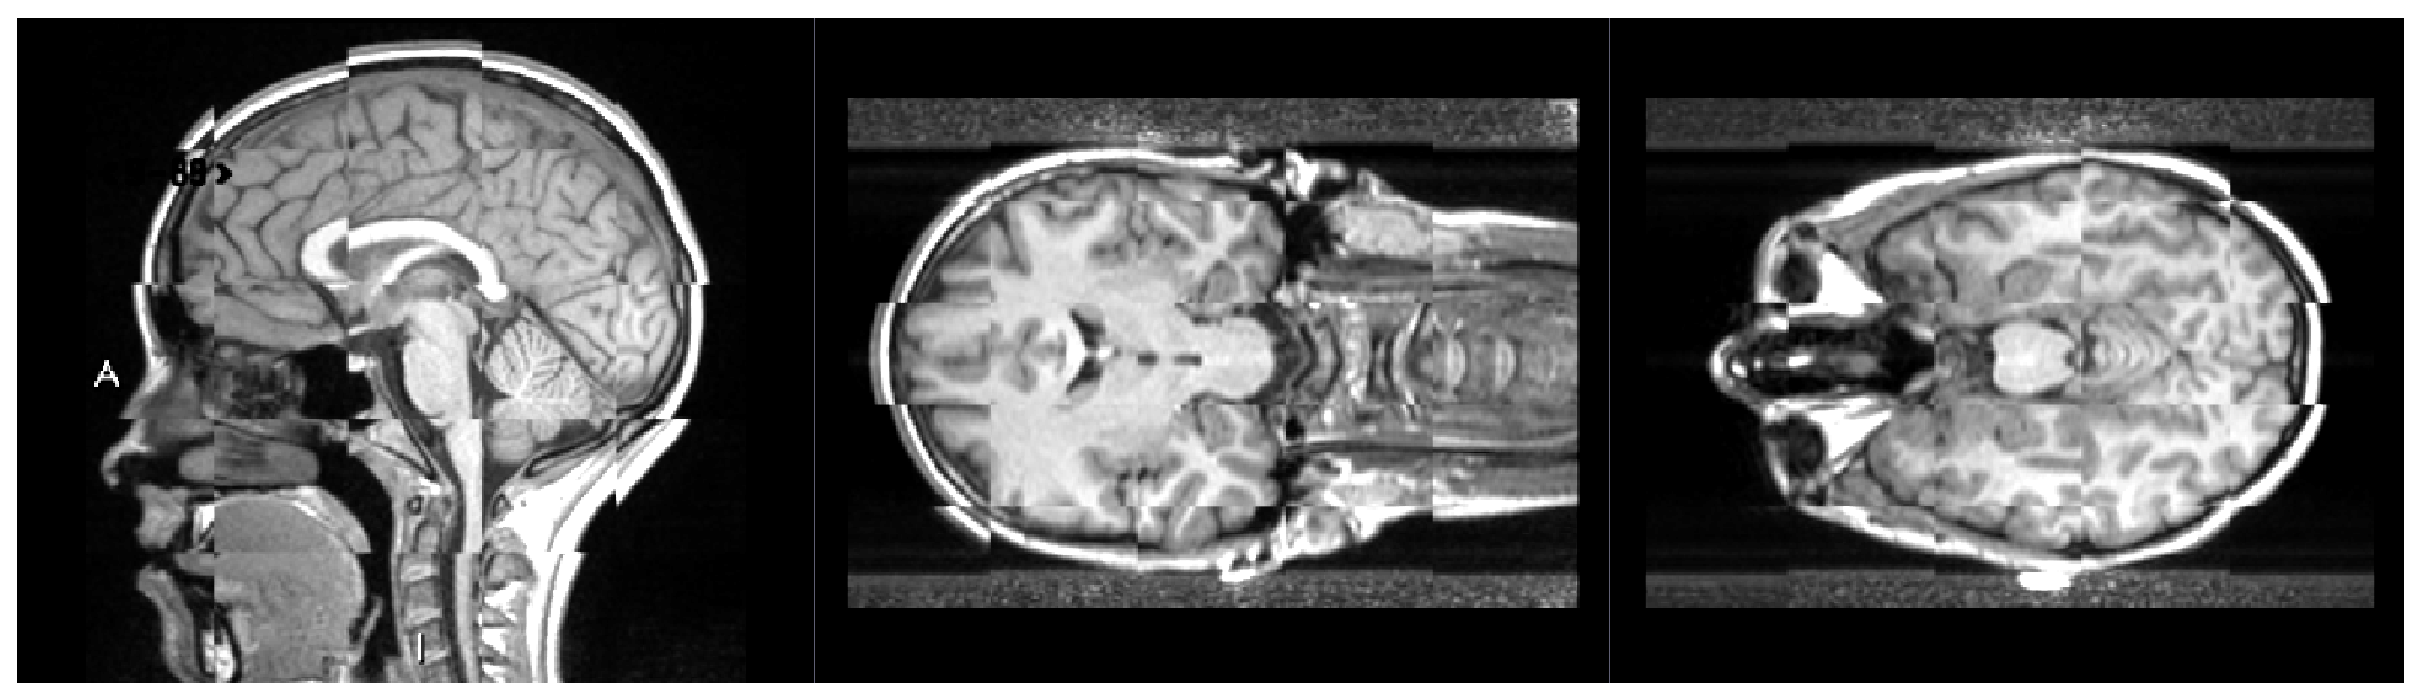
\includegraphics[scale=0.3]{before_registration.eps}
  \caption{Comparison of volumes before registration}
  \label{before_reg}
\end{figure}


\begin{figure}[htb]
  \centering
  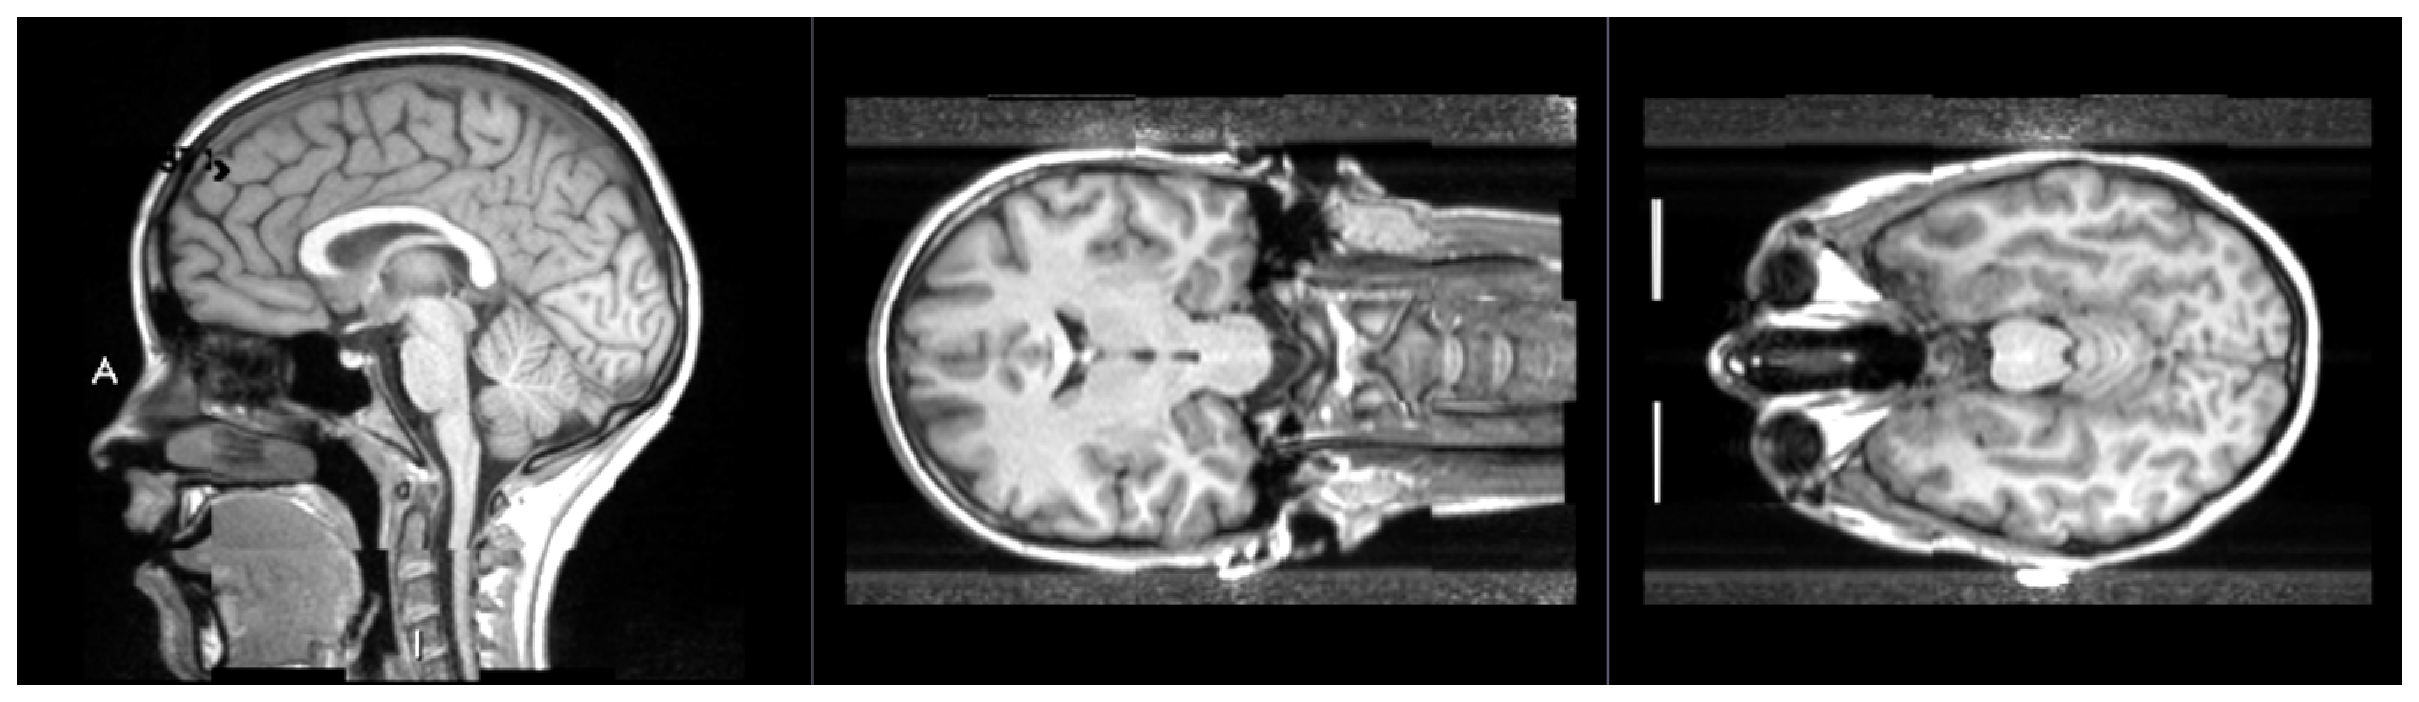
\includegraphics[scale=0.3]{after_registration.eps}
  \caption{Comparison of volumes after registration}
  \label{after_reg}
\end{figure}

The second volume has been modified using affine registration so that
the comparison between both volumes becomes much easier.\\

According to \cite{zitova}, the majority of the registration methods consist of the following steps:
\begin{enumerate}
\item \textit{Feature detection:} Salient and distinctive objects are detected.
\item \textit{Feature matching:} The correspondence between the features detected in the sensed image and those detected in the reference image is established.
\item \textit{Transform model estimation:} The type and parameters of the mapping functions are estimated. These functions align the sensed image with the reference image.
\item \textit{Image resampling and transformation:} The sensed image is transformed by means of the mapping functions.
\end{enumerate}


\subsection{Registration Methods used}
There are many different methods to accomplish registration between
images or volumes. In this project only a few of these methods were
used based on experiments performed with some of the available
methods. The chosen procedures were the ones that behaved better
under the specific conditions of this work.


\subsubsection{Affine Registration}
In geometry, an \textit{affine transformation} or an \textit{affinity}
is a transformation which preserves straight lines (i.e., all points
lying on a line initially still lie on a line after the
transformation) and ratios of distances between points lying on a
straight line. It does not necessarily preserve angles or lengths, but
does have the property that sets of parallel lines will remain
parallel to each other after an affine transformation \cite{affine_t}. \\

The implementation of affine registration used during this project is
the one included in \textit{3D Slicer} version 4.1. 

The application is able to register two images together using an
affine transform and mutual information, and it allows the user to
modify quite a few parameters
in order to obtain the expected result.\\

If you would like to know more about this implementation of affine
registration please refer to the module webpage:

\url{http://wiki.slicer.org/slicerWiki/index.php/Documentation/4.1/Modules/AffineRegistration}

\subsubsection{B-Spline Registration}
In the mathematical subfield of numerical analysis, a
\textit{B-spline} is a spline function that has minimal support with
respect to a given degree, smoothness, and domain partition.

However, in computer graphics, the term \textit{B-spline} frequently
refers to a spline curve parametrized by spline functions that are
expressed as linear combinations of \textit{B-splines} (in the
mathematical sense explained above) \cite{bspline}.\\

Just like in the case of affine registration, the implementation of
B-Spline registration used during this project is the one included in
\textit{3D Slicer} version 4.1. 

The application divides the volumes into a grid of user-defined size
in which each line is a B-spline that will be modified by the
registration to create a transform that aligns the two volumes.\\

If you would like to know more about this implementation of B-spline
registration please refer to the module webpage:

\url{http://wiki.slicer.org/slicerWiki/index.php/Documentation/4.1/Modules/BSplineDeformableRegistration}


\subsubsection{BRAINS Demon Warp Registration}
As with the registration methods explained before, \textit{BRAINS
  Demon Warp} registration is implemented as a module in \textit{3D
  Slicer} version
4.1.\\

The module works by using the ITK filter based on Thirion's Demons
algorithm, in which the main idea is to consider the objects
boundaries in one image as semi-permeable membranes and to let the
other image, considered as a deformable grid model, diffuse through
these interfaces, by the action of effectors situated within the
membranes. \cite{thirion}.

An important characteristic of this implementation, that was
particularly useful for this project, is that it can produce a
\textit{deformation field} as the output of the registration. A
deformation field is a vector image in which each point is a vector
that indicates the amount of deformation necessary
at that point in order to align the volumes.\\


If you would like to know more about the implementation of
\textit{BRAINS Demon Warp} registration please refer to the module
webpage:

\url{http://wiki.slicer.org/slicerWiki/index.php/Documentation/4.1/Modules/BRAINSDemonWarp}


\section{Morphometry}
Morphometry refers to the measurement of external form. More
specifically, \textit{brain morphometry} is concerned with the
measurement of brain structures and changes thereof during
development, aging, learning, disease and evolution. Its goal is to
derive specific information from noninvasive neuroimaging data of live
brains, typically obtained from magnetic resonance imaging (MRI); and
to quantify the anatomical features of the brain in terms of shape,
mass and volume \cite{brmorph}.

\subsection{Voxel-based Morphometry}

\subsection{Tensor-based Morphometry}
\subsection{Deformation-based Morphometry}